\documentclass{article}
\usepackage[utf8]{inputenc}
\usepackage{graphicx}
\usepackage{mathtools} 
\usepackage{textcomp}
\usepackage{titling}
\usepackage{subfig}
\usepackage{amsmath}
\usepackage[parfill]{parskip}
\usepackage{xcolor}
\definecolor{LightGray}{gray}{0.9}
\usepackage{titlesec}
\setcounter{secnumdepth}{4}
\usepackage[a4paper,left=1cm,right=1cm,top=1cm,bottom=1.5cm,]{geometry}
\usepackage{eqparbox}
\usepackage{enumitem}
\usepackage{graphicx}
\newcommand*{\Scale}[2][4]{\scalebox{#1}{\ensuremath{#2}}}%
\usepackage{centernot}

\title{\vspace{-2cm} EE4218 PP3 - Placement/Routing}
\date{\vspace{-5ex}}

\begin{document}
\maketitle

\section{Notes}
\begin{figure}[htp]
    \centering
    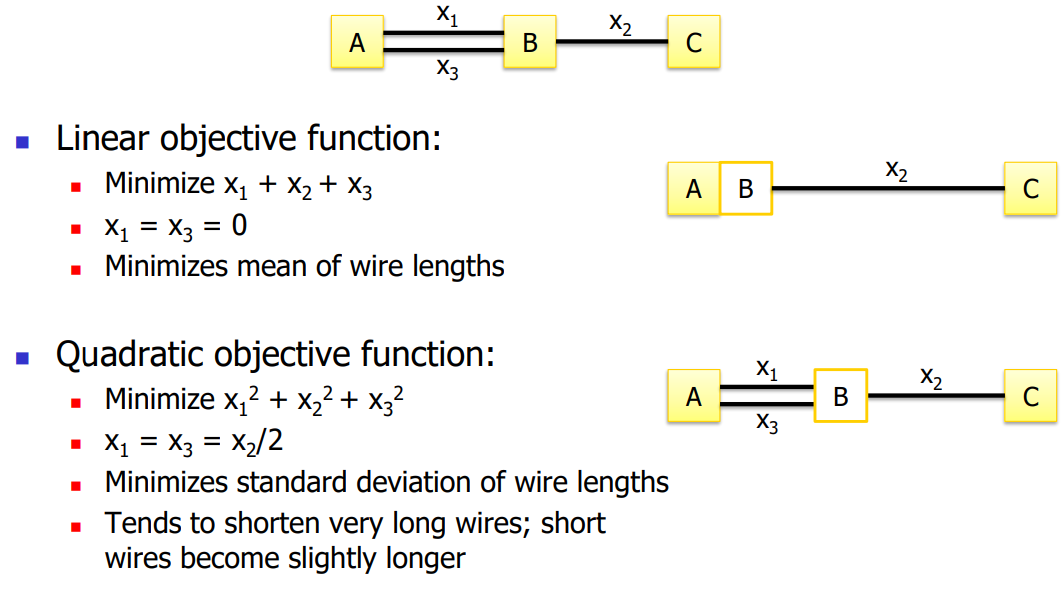
\includegraphics[width=8cm, scale=1]{analyticalPlacement.PNG}
    \caption{Analytical Placement}
\end{figure}

\begin{minipage}[t]{0.5\textwidth}
    \centering
    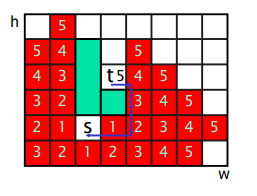
\includegraphics[width=7cm, scale=1]{mazeRouting1.PNG}
    \captionof{figure}{Two terminals}
\end{minipage}%
\begin{minipage}[t]{0.5\textwidth}
    \centering
    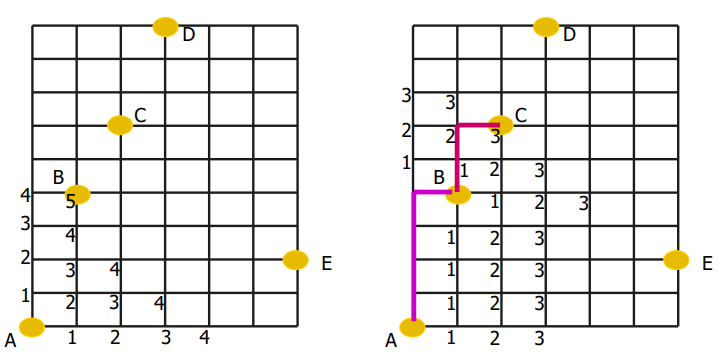
\includegraphics[width=10cm, scale=1]{mazeRouting2.PNG}
    \captionof{figure}{More than two terminals}
\end{minipage}%

\begin{itemize}
    \item Suppose that we have to route from some source node $S$, to two destination nodes $D_{1}$ and $D_{2}$.
    \item Assume that we route to $D_{1}$ first, and there $\exists$ two equally optimal paths $p_{1}$ and $p_{2}$ which route $S$ to $D_{1}$
    \item Then, it is \textbf{not true} that utilizing utilizing $p_{1}$ to route to $D{2}$ is \textbf{always as} optimal as utilizing $p_{2}$ to route to $D_{2}$
\end{itemize}

\begin{minipage}[t]{0.5\textwidth}
    \centering
    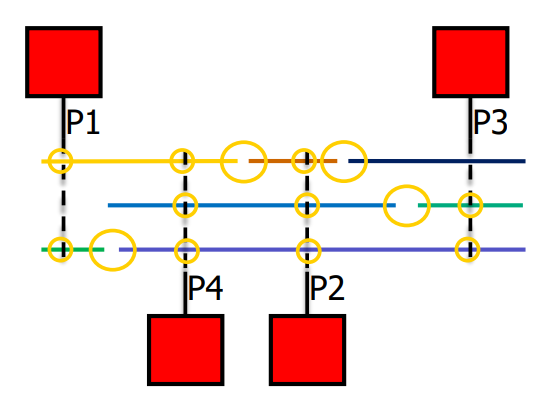
\includegraphics[width=8cm, scale=1]{routing1.PNG}
    \captionof{figure}{Connection required from P1 to P2, P3 to P4}
\end{minipage}%
\begin{minipage}[t]{0.5\textwidth}
    \centering
    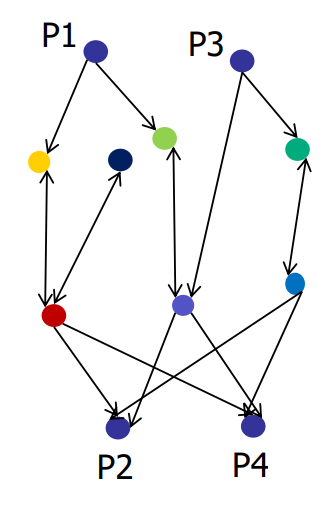
\includegraphics[width=4cm, scale=1]{routing2.PNG}
    \captionof{figure}{Graph}
\end{minipage}%

\begin{itemize}
    \item \textit{Criticality of connection} from source ($S$) to target ($T$) given by \dots
        \begin{itemize}
            \item $Crit(S,T) = 1 - \frac{Slack(S,T)}{D_{max}}$
            \item $Slack(S,T)$ is amount of delay that can be added to connection, before it affects critical path delay
            \item $D_{max}$ is delay of circuit's critical path
        \end{itemize}
    \item \textit{Cost} of using routing resource node $n$, as part of \textit{connection} $(S,T)$ given by \dots
        \begin{itemize}
            \item $Cost(n) = Crit(S,T) \cdot delay(n) + (1-Crit(S,T)) \cdot (delay(n)+h(n))p(n)$
            \item $h(n)$ is historic congestion (eg. moving average of past three iterations)
            \item $p(n)$ is present congestion of node (ie. how many nets using node)
        \end{itemize}
\end{itemize}


\end{document}